\documentclass{article} % For LaTeX2e
\usepackage{iclr2018_conference,times}
\usepackage{hyperref}
\usepackage{url}
\usepackage{natbib}
\usepackage{amsfonts}
\usepackage{amsmath}
\usepackage{graphicx}
\usepackage{subcaption}
\graphicspath{ {images/} }	

\title{ImgPCA \\ A data visualization tool for PCA Analysis \\ MAI718 3/2017 Final project}

% Authors must not appear in the submitted version. They should be hidden
% as long as the \iclrfinalcopy macro remains commented out below.
% Non-anonymous submissions will be rejected without review.

\author{Roberto Stelling \thanks{ PPGI/UFRJ Graduate Student, \href{http://stelling.cc}{http://stelling.cc}.} \\
PPGI - 117.335.792\\
Universidade Federal do Rio de Janeiro\\
Rio de Janeiro, RJ 21941-916, Brazil \\
\texttt{roberto@stelling.cc}
}

% The \author macro works with any number of authors. There are two commands
% used to separate the names and addresses of multiple authors: \And and \AND.
%
% Using \And between authors leaves it to \LaTeX{} to determine where to break
% the lines. Using \AND forces a linebreak at that point. So, if \LaTeX{}
% puts 3 of 4 authors names on the first line, and the last on the second
% line, try using \AND instead of \And before the third author name.

\newcommand{\fix}{\marginpar{FIX}}
\newcommand{\new}{\marginpar{NEW}}

\iclrfinalcopy % Uncomment for camera-ready version, but NOT for submission.
\begin{document}
\maketitle
\pagestyle{plain}

\begin{abstract}
Traditionally PCA Analysis for dimension reduction in images is performed without a systematic visual aid approach. This paper describes a data visualization tool for PCA Analysis implemented in JavaScript aiming to improve the analyst decision process.
\end{abstract}

\section{Problem description}
There are many reasons to reduce a data set, some examples are: noise reduction, outlier removal, lossy image compression or even as a preliminary step in various types of data exploration and data analysis.\par
Principal component analysis (PCA) can be used as a lossy image compression solution, as you can apply PCA on a set of images of a data set and reduce its dimensionality with a certain, desirably controllable, loss of precision. Of course, one want to loose as little precision as possible while compressing as much as possible.With images, the main difficulty resides in the trade off between compression and precision: how many dimensions can be thrown away making sure that the resulting images still retain the desired level of quality or sharpness? Is there a general rule where you can certainly decide how many dimensions will be cut off the original data set? Of course, the type and amount of data available for compression, the data set, has a big influence on the precise point where the cut will happen, but can the analyst decide simply on the number of dimensions or amount of variance that will be thrown away and be sure that the results will be satisfactory? We propose that using a visual helping tool during the decision process can have a positive impact on the cut off selection.

\section{Brief introduction to PCA}
\subsection{Objective}
According to \citet{jolliffe1986principal}, the central idea of principal component analysis (PCA) is to reduce the dimensionality of a data set in which there are a large number of interrelated variables, while retaining as much as possible of the variation present in the data set.\par
This reduction is achieved by transforming the data set into a new set of variables, the principal components, which are not correlated, and which are ordered so that the first few retain most of the variation present in all the original variables.\par
\subsection{Brief History of PCA}
Principal component analysis was first described by \citet{pearson1901principal} and later developed independently by \citet{hotelling1933analysis} \citep{jolliffe1986principal}.\par
\citet{preisendorfer1988principal} state that in 1873, the Italian geometer Beltrami, formulated a modern form of the resolution of a general square matrix into its singular value decomposition (SVD), the decomposition that stands at the base of PCA.\par
\citet{craw1992face} describe a method for face recognition using principal component analisys, showing that PCA can be used as an effective tool in image analysis.
\subsection{Intuition}
PCA can be thought of as the problem of fitting an $n$-dimensional ellipsoid to the $m$-dimensional data, where $n<=m$ and each axis of the ellipsoid represents a principal component. The larger the axis of a component, the larger the variance for that component. So, the objective of PCA is to build a transformation of $m$-dimensional space to $n$-dimensional space while preserving most of the the $m$-dimensional space variance. To find that transformation and the components, we compute the singular value decomposition of the data. The singular value decomposition will provide a computationally efficient method of finding the principal components and the scaled versions of the principal component scores.
\subsection{Singular Value Decomposition}
Given an arbitrary $D_{m\times n}$ matrix, then $D$ can be written as
\begin{equation} \label{eq1}
D_{m\times n}=U_{m\times r}S_{r\times r}V_{r\times n}^T
\end{equation}
where
\begin{enumerate}
\item[(i)] $U$ and $V$, each of which with orthonormal\footnote{both orthogonal and normalized} columns so that $U^TU=I_{r}$, $V^TV=I_{r}$;
\item[(ii)] $S$ is a diagonal matrix;
\item[(iii)] $r$ is the rank\footnote{corresponds to the maximal number of linearly independent columns of D} of $D$.
\end{enumerate}
$S$ is a diagonal matrix such as:
\[
  S =
  \begin{bmatrix}
    s_{1} & & \\
    & \ddots & \\
    & & s_{r}
  \end{bmatrix}
\]
Where $s_{1}$ to $s_{r}$ are the principal components scores and $s_{1} >= s_{2} >= ... >= s_{r-1} >= s_{r}$.\par
$U$ is the eigenvector matrix, with eigenvectors ordered by the component scores, their eigenvalues.
\subsection{Principal Component Analysis}
To apply PCA we will use equation (\ref{eq1}) from the singular value decomposition and apply it to the covariance matrix $\Sigma$ of a data set. If the data set $D$ has dimensions ${m\times n}$ then the covariance matrix $\Sigma$ will be a symmetrical square matrix of dimensions $n\times n$. So
\begin{equation}\label{eq2}
\Sigma_{n\times n} = U_{n\times n}S_{n\times n}V_{n\times n}^T
\end{equation}
Where
\begin{itemize}
\item $U$ is orthonormal and holds $\Sigma$ eigenvectors
\item $S$ is a diagonal matrix with $s_1 ... s_n$ as the descending ordered eigenvalues.
\end{itemize}
As $U$ is orthonormal then we can transform the original $D$ data set into $P$
\[ P_{m\times n} = D_{m\times n}U_{n\times n} \] and restore it back with:
\[P U^T = DUU^T = DI_{n} = D\]
$P$ is a transformation of $D$ that retains all the information of the original data set.

\section{PCA for image compression}
A computer image is usually thought of as a two dimensional matrix, with $m$ lines and $n$ columns representing the horizontal and vertical pixels of the image. A simpler, albeit equally meaningful, representation is a single vector with $m\times n$ cells for the whole image. The content of each cell, in either representation, depends on the selected image mode. For example: RGB, RGB grayscale, CMYK, etc. For the purposes of the following argument and the solution implementation, we assume that each cell is an integer between 0 and 255, representing the grayscale RGB value of the corresponding pixel. We will also assume that our data set has $m$ samples of $n$ pixels; if $h$ is the number of horizontal pixels and $v$ is the number of vertical pixels, then $n=h\times v$.\par
Lets assume that $D$ is a data set with $m$ images where each image has $n$ pixels. Computationally the method can work even if $m<n$ but it is recommended that $m >= n$, as that will result in better compression gains and finer eigenvector tuning.\par
Given that $D_{m\times n}$ is a data set with $m$ data points $\in \mathbb{R}^n$ where $m >= n$. Then we define ${D}_{m\times n}^*$ as the normalized data set, \[D^* = \frac{D-\overline{D}}{s}\] 
where $\overline{D}$ is the mean of $D$ and $s$ is the sample standard deviation of D. Let $\Sigma_{n\times n}$ be the covariance matrix of $D^{*}_{m\times n}$ \[\Sigma = \frac{1}{m}D^{*T}D^*\] Then, according to (\ref{eq1}) and (\ref{eq2}), the singular value decomposition of $\Sigma$ is: 
\begin{equation}\label{eq3}
\Sigma = US V^T
\end{equation}
where:
\begin{itemize}
\item $U$ is an $n\times n$ orthonormal matrix
\item $S$ is an $n\times n$ diagonal matrix with non-negative numbers on the diagonal
\item $V$ is an $n\times n$ unitary matrix and $V^T$ is $V$ transposed.
\end{itemize}

\subsection{Reducing dimensions}
Given the original data set, $D_{m\times n}$ and $U_{n\times n}$ obtained from $\Sigma$ as per (\ref{eq3}), then we can build a new reduced data set $P_{m\times k}$ with the first $k<n$ eigenvectors. This new data set is computed as:
\begin{equation}\label{eq4}
P_{m\times k} = D_{m\times n} U_{n\times k}
\end{equation}
where $U_{n\times k}$, or $U_k$, is the eigenvector matrix truncated to the first $k$ eigenvectors. The information contained on the truncated $(n-k)$ columns is lost in this transformation.
\subsection{Restoring data}
The transformation in (\ref{eq4}) is lossy, meaning that the information on the truncated $n-k$ columns is utterly lost during the transformation. Although it is possible to restore $P$ back to $D$ dimensions, the result will not be exactly $D$ but rather an approximation of $D$. The whole rationale of using PCA for image compression is that the last $n-k$ eigenvectors will hold as little variance as possible and the recovered images will be an acceptable approximation of the original images.
To transform $P$ back into $D$ space we compute \[P_{m\times k}U_{k\times n}^T = D_{m\times n}U_{n\times k}U_{k\times n}^T \approx D_{m\times n}\]
\section{How to select the number of components to retain}
The problem of selecting how many components to retain is not new, \citet{zwick1986comparison}, present the results of a Monte Carlo evaluation of five methods that have been proposed for determining how many factors or components to retain: Horn's parallel analysis, Velicer's minimum average partial, Cattell's scree test, Bartlett's chi-square test, and Kaiser's eigenvalue greater than $1.0$ rule. 
The determination of the number of components or factors to retain is likely to be the most important decision a researcher will make \citep{zwick1986comparison}.\par

We propose that a graphical supporting tool, with a graph similar to Cattell's scree plot but displaying $\log_{10} eigenvalues$ instead of $eigenvalues$, plus on the fly representations of a subset of the compressed images, and a subset of the eigenimages, can be instrumental in the decision of how many dimensions must be retained. We suggest that the use of eigenimages can increase the analyst understanding of the variation and trends of main eigenvectors of the data set.\par
The number of dimensions to retain will eventually be a decision based on the supporting graphs and the recovered images. We include a couple of numeric measures on the cut off point:
\begin{itemize}
\item Accumulated variation retained.
\item Number of components retained.
\item Component score on the cut off point, the cut off point eigenvalue.
\end{itemize}
If we were to use a rule similar to Kaiser's Rule\footnote{Eigenvalues greater than one}, based on our experience with the proposed tool with $32\times 32$ grayscale images, then we would suggest a $\frac{1}{10}$ Kaiser's Rule: eigenvalues greater than $0.1$. Trials with a few data sets suggest that a "\emph{One Tenth Kaiser's Rule}" with eigenvalues $> 0.1$ is a reasonable trade off between compression and sharpness.

%\begin{figure}[h]
%\begin{center}
%%\framebox[4.0in]{$\;$}
%\fbox{\rule[-.5cm]{0cm}{4cm} \rule[-.5cm]{4cm}{0cm}}
%\end{center}
%\caption{Sample figure caption.}
%\end{figure}

\begin{figure}[h]
\begin{center}
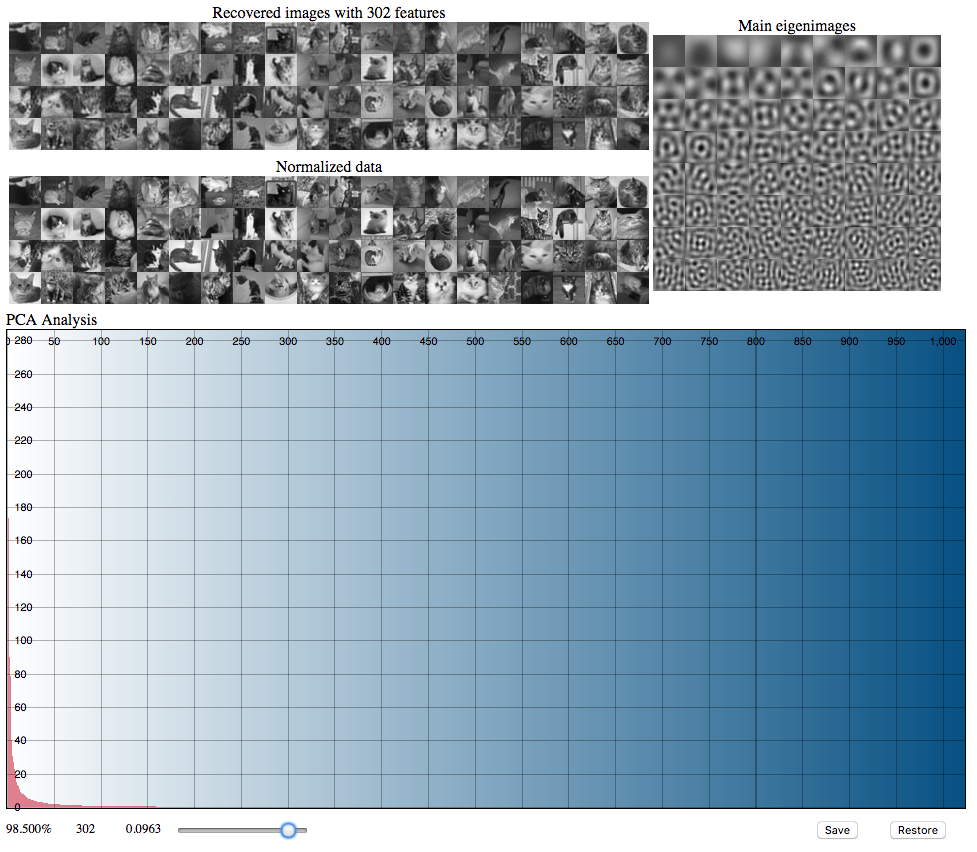
\includegraphics[width=\textwidth]{imgPca.png}
\end{center}
\caption{ImgPCA screenshot with a signature $eigenvalues \times \#of components$ curve.}
\end{figure}
Note that the Kaiser's Rule cut occurs exactly where the graph crosses $0$ ($\log_{10} eigenvalue = 0$) and that our "\emph{One Tenth Kaiser's Rule}" occurs when $\log_{10} eigenvalue = -1$.
\section{Examples}
For the next few examples we are going to use a subset of CIFAR-10 (\citet{krizhevsky2009learning}, chapter 3) images modified to fit our purposes. CIFAR-10 is a collection of $32\times 32$ color images that are available in python, Matlab and binary versions. We converted CIFAR-10 images to grayscale (see \nameref{materials}), rotated the images $90$ degrees to produce the input files for our usage.\par

\begin{figure}[h]
\centering
\begin{subfigure}{.5\textwidth}
  \centering
  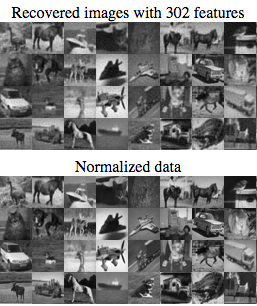
\includegraphics[width=.9\linewidth]{CIFAR10All1024RecoveredNormalized}
  \caption{$302$ components}
  \label{fig:cifarall302}
\end{subfigure}%
\begin{subfigure}{.5\textwidth}
  \centering
  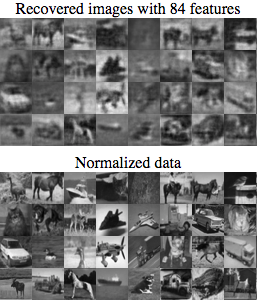
\includegraphics[width=.9\linewidth]{CIFAR10All1024RecoveredNormalized84}
  \caption{$84$ components}
  \label{fig:cifarall84}
\end{subfigure}
\caption{CIFAR-10 images recovered using "\emph{One Tenth}" (\ref{fig:cifarall302}) and regular Kaiser's rule (\ref{fig:cifarall84}).}
\label{fig:sampleCifar10}
\end{figure}

For the first example we will exam $1024$ images with $1024$ ($32\times 32$) pixels from all CIFAR-10 classes, in the order they appear on the original file. Figure \ref{fig:sampleCifar10} displays the same set of images, recovered with $302$ and $84$ components. The $302$ components represent $98.786\%$ of variance, with the smallest component score being $0.1011$, following our "\emph{One Tenth Kaiser's Rule}". There are a few artifacts on the recovered images but the results seems to be visually satisfactory.\par

\begin{figure}[h]
\centering
\begin{subfigure}{.5\textwidth}
  \centering
  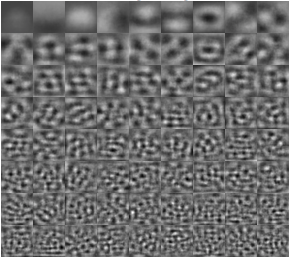
\includegraphics[width=.9\linewidth]{CIFAR10All1024Eigenimages}
  \caption{From $1024$ images}
  \label{fig:eigenImagesAll1024}
\end{subfigure}%
\begin{subfigure}{.5\textwidth}
  \centering
  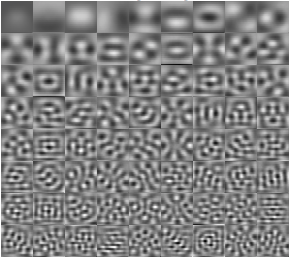
\includegraphics[width=.9\linewidth]{CIFAR10All15000Eigenimages}
  \caption{From $15000$ images}
  \label{fig:eigenImagesAll15000}
\end{subfigure}
\caption{Eigenimages generated from $1024$ and $15000$ images of all CIFAR-10 classes.}
\label{fig:eigenImagesAll}
\end{figure}

If we increase the number of images on the data set, from $1024$ to $15000$ images then we notice a few changes on ImgPCA graphics display, the most notable visual difference is the definition and ordering of the eigenimages.\par
Figure \ref{fig:eigenImagesAll} shows the first $72$ eigenimages generated from data sets of size $1024$ (Figure \ref{fig:eigenImagesAll1024}) and $15000$ (Figure \ref{fig:eigenImagesAll15000}) images of all CIFAR-10 classes. The eigenimages reveal some characteristics of the images on the dataset: centrality of subject, dark central subject on a clear image, clear central subject on a dark image, left to right symmetry, bottom to top symmetry among others. It is not surprising that the ordering of the eigenimages changes when we increase or decrease the number of images of our test sample but the improvement of eigenimage definition and sharpness when the size of the data set increases is striking.

\begin{figure}[h]
\centering
\begin{subfigure}{.5\textwidth}
  \centering
  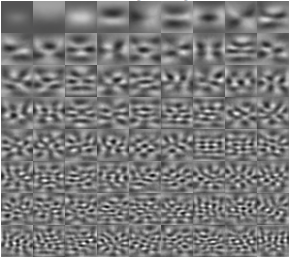
\includegraphics[width=.9\linewidth]{CIFAR10C05000Eigenimages}
  \caption{Class 0 - Planes}
  \label{fig:eigenImagesC0}
\end{subfigure}%
\begin{subfigure}{.5\textwidth}
  \centering
  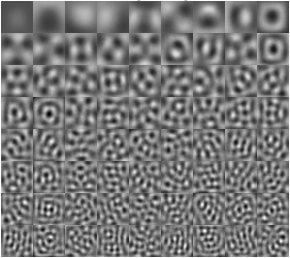
\includegraphics[width=.9\linewidth]{CIFAR10C35000Eigenimages}
  \caption{Class 3 - Cats}
  \label{fig:eigenImagesC3}
\end{subfigure}
\caption{Eigenimages generated from $5000$ images of two different classes.}
\label{fig:eigenImagesC0C3}
\end{figure}

This CIFAR-10 subset includes images from all $10$ categories (numbered from $0$ to $9$) and has as much variance as possible given the chosen subject of the data set. On Figure \ref{fig:eigenImagesC0C3} we can see the eigenimages generated from 5000 images of CIFAR-10 class 0 (\ref{fig:eigenImagesC0}) and CIFAR-10 class 3 (\ref{fig:eigenImagesC3}).\par Not only the eigenimages are different but one can almost see vestigial planes on \ref{fig:eigenImagesC0} and vestigial cats on \ref{fig:eigenImagesC3}.
This effect, applied to faces, or eigenfaces, was observed and developed by \citet{sirovich1987low}.

\section{Materials and Methods}\label{materials}
The code for the implementation and supporting documents can be found at \citet{Stelling:aa}.

\section{Citations, figures, tables, references}
\label{others}

These instructions apply to everyone, regardless of the formatter being used.

\subsection{Citations within the text}


Citations within the text should be based on the \texttt{natbib} package
and include the authors' last names and year (with the ``et~al.'' construct
for more than two authors). When the authors or the publication are
included in the sentence, the citation should not be in parenthesis (as
in ``See \citet{Goodfellow:2016aa} for more information.''). Otherwise, the citation
should be in parenthesis (as in ``Deep learning shows promise to make progress towards AI~\citep{Goodfellow:2016aa}.'').

The corresponding references are to be listed in alphabetical order of
authors, in the \textsc{References} section. As to the format of the
references themselves, any style is acceptable as long as it is used
consistently.


\subsection{Tables}

All tables must be centered, neat, clean and legible. Do not use hand-drawn
tables. The table number and title always appear before the table. See
Table~\ref{sample-table}.

Place one line space before the table title, one line space after the table
title, and one line space after the table. The table title must be lower case
(except for first word and proper nouns); tables are numbered consecutively.

\begin{table}[h]
\caption{Sample table title}
\label{sample-table}
\begin{center}
\begin{tabular}{ll}
\multicolumn{1}{c}{\bf PART}  &\multicolumn{1}{c}{\bf DESCRIPTION}
\\ \hline \\
Dendrite         &Input terminal \\
Axon             &Output terminal \\
Soma             &Cell body (contains cell nucleus) \\
\end{tabular}
\end{center}
\end{table}




\subsubsection*{Acknowledgments}
I'd wish to thank the whole of the MAI718/2017-3 class for their invaluable input during preliminary presentations of the current work. Your ideas, discussions and critiques where instrumental in improving the foundations of this work. 

I'd specially like to thank PPGI/UFRJ for letting me use their computer laboratory for the duration of the term. Without that access I wouldn't have the means to work on this project with the intensity it required.

\bibliography{imgPCA}
\bibliographystyle{iclr2018_conference}

\end{document}
